\documentclass[oneside,final,12pt]{article}

\usepackage[T2A]{fontenc}
%\usepackage[utf8]{inputenc}   % older versions of ucs package
\usepackage[utf8x]{inputenc}  % more recent versions (at least>=2004-17-10)
\usepackage[russian]{babel}
\usepackage{graphicx}
\usepackage{vmargin}
\setpapersize{A4}
\setmarginsrb{3cm}{2cm}{1.5cm}{2cm}{0pt}{0mm}{0pt}{13mm}
\usepackage{indentfirst}
\usepackage[footnotesize]{caption2}
\usepackage{alltt}

\sloppy

% Параметры страницы
\textheight=24cm
\textwidth=16cm
\footnotesep=3ex
\raggedbottom
\tolerance 3000
% подавить эффект "висячих стpок"
\clubpenalty=10000
\widowpenalty=10000
\renewcommand{\baselinestretch}{1.1}
\renewcommand{\baselinestretch}{1.5} %для печати с большим интервалом

\begin{document}

\begin{titlepage}
\begin{center}

    \bigskip
    
\includegraphics[width=100mm]{msu.eps}

    \bigskip
    Московский государственный университет имени М. В. Ломоносова\\
    Факультет вычислительной математики и кибернетики\\[10mm]
   Отчет по заданию практикума \\[5mm]   
    \textsf{\large\bfseries
        Моделирование обслуживания в филиале банка
    }\\[50mm]

   
    \begin{flushright}
        \parbox{0.4\textwidth}{
            студент 4 курса 424 группы\\
            \emph{Зуев Кирилл Александрович}\\[5mm]
        }
    \end{flushright}

    \vspace{\fill}
    Москва, 2018
\end{center}
\end{titlepage}

\newpage
\renewcommand{\contentsname}{Содержание}
\tableofcontents

\newpage
\section{Уточнение постановки задачи}

Необходимо создать компьютерную модель обслуживания потока заявок, поступающих от клиентов банка, несколькими клерками ($2 \leq N \leq 7$) в одном из филиалов банка. Известно недельное расписание работы филиала банка: 5 дней по 8 часов и один день --- 6 часов, возможны перерывы на обед.

При моделировании работы заявки на обслуживание (т.е. приход клиентов) поступают случайным образом. Случайной величиной является отрезок времени между последовательным появлением двух заявок (например, от 0 до 10 минут). Длительность обслуживания каждой заявки --- также случайное число в некотором диапазоне (например, от 2 до 30 минут), но длительность не зависит от входного потока заявок. Еще одна случайная величина --- прибыль, получаемая банком от обслуживания клиента, она варьируется в пределах от 3 тыс. до 50 тыс. рублей.

Поступившие заявки (клиенты) образуют общую очередь, максимальная длина которой --- $K$ человек ($10 \leq K \leq 25$). Если очередь достигла такой длины, то вновь прибывающие клиенты уходят --- тем самым банк теряет своих потенциальных клиентов.

Клиенты банка ожидают своей очереди на обслуживание в общем зале с информационным табло, на котором высвечиваются номер клиента, взятого только что на обслуживание, и номер места клерка, обслуживающего этого клиента. В каждый день работы филиала заявки на обслуживание нумеруются последовательно, начиная с 1, по мере их прихода в банк.

Цель моделирования работы банка --- определение прибыли банка и ее зависимости от числа работающих клерков; выявление <<узких>> мест в работе банка: нехватки клерков (возможное следствие этого --- потеря клиентов), простой клерков (следствие --- лишние траты на их зарплату). Прибыль высчитывается с учетом дневной зарплаты каждого клерка (2 тыс. руб.).

Период моделирования --- месяц, шаг моделирования интервал времени от 10 минут до 1 часа. Следует включить в параметры моделирования: числа $N$ и $K$, шаг моделирования, диапазоны разброса случайных величин промежутка между приходом клиентов и время их обслуживания.

Визуализация моделируемого процесса должна предусматривать показ текущей ситуации в банке, в том числе скопившуюся очередь, занятость клерков, появление новых и уход обслуженных клиентов, информационное табло. Следует предусмотреть вывод в ходе моделирования и по его окончании подсчитанной статистики: количества обслуженных и потерянных клиентов, а также полученную банком прибыль.

\newpage
\section{Диаграмма основных классов}

 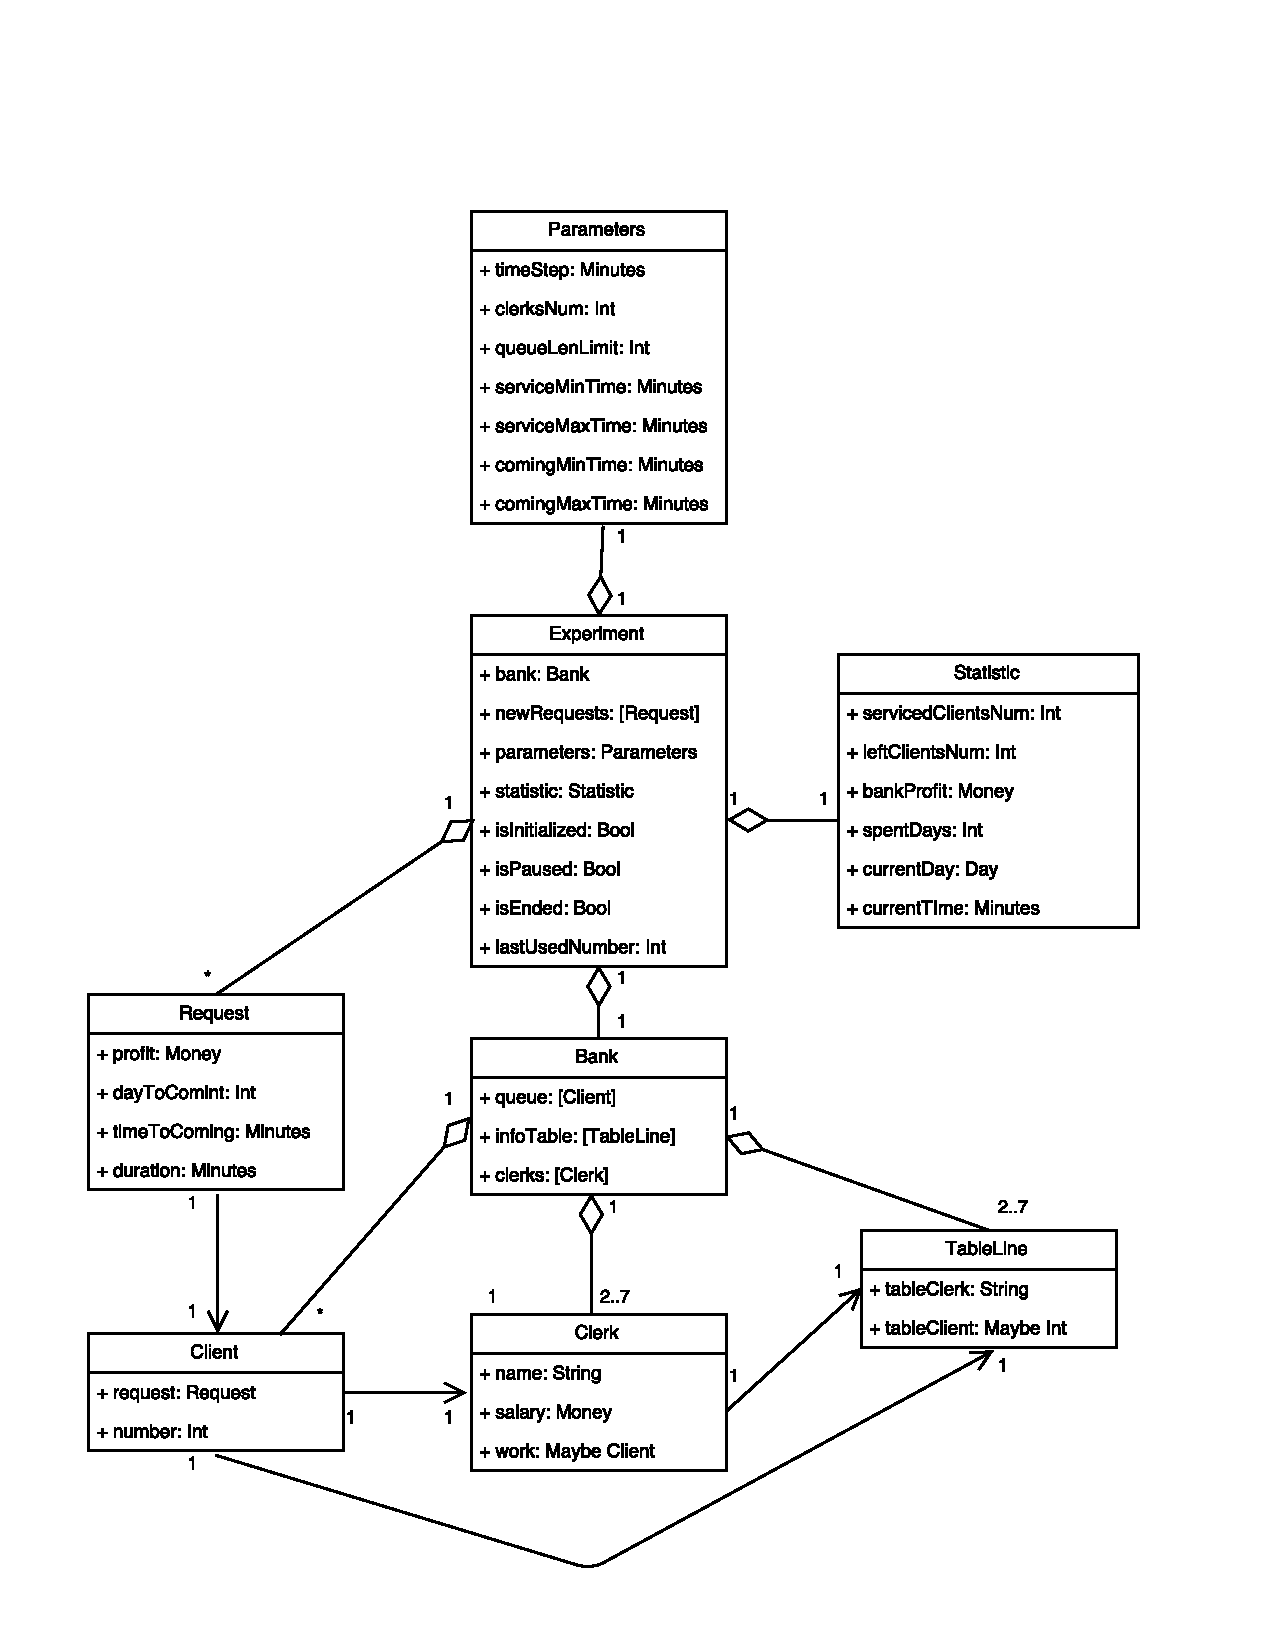
\includegraphics[width=180mm]{classes.pdf}
\newpage

\section{Спецификации интерфейса}

\begin{alltt}
-- * Эксперимент
data Experiment = Experiment
\{ bank           :: Bank       -- ^ банк
	, newRequests    :: [Request]  -- ^ поток поступающих заявок
	, parameters     :: Parameters -- ^ параметры
	, statistic      :: Statistic  -- ^ статистика
	, isInitialized  :: Bool       -- ^ инициализирован ли
	, isPaused       :: Bool       -- ^ поставлен ли на паузу
	, isEnded        :: Bool       -- ^ закончен ли
	, lastUsedNumber :: Int        -- ^ последний использованный номер клиента
\} deriving (Eq)

class ExperimentClass experiment where
-- | Инициализировать эксперимент
initExperiment      :: experiment
-- | Изменить параметр
changeParameter     :: ParametersField -> ChangeAction -> experiment -> experiment
-- | Начать эксперимент
startExperiment     :: StdGen -> experiment -> experiment
-- | Продолжить/приостановить эксперимент
playPauseExperiment :: experiment -> experiment
-- | Сбросить эскперимент
resetExperiment     :: experiment
-- | Перейти к концу эксперимента
finishExperiment    :: experiment -> experiment
-- | Добавить заявки в очередь в виде клиентов и обновить статистику.
-- Учитываются ушедшие клиенты.
addToQueue          :: [Request] -> experiment -> experiment
-- | Уход клиентов из очереди
leftFromQueue       :: experiment -> experiment
-- | Занять при возможности свободных клерков
setWorkToClerks     :: experiment -> experiment
-- | Обновить очередь клиентов
updateClients       :: experiment -> experiment
-- | Обновить состояние клерков
updateClerks        :: experiment -> experiment
-- | Добавить клиентов в очередь.
addClients          :: [Request] -> experiment -> experiment
-- | Моделирование заданного промежутка времени.
addTime             :: Minutes -> experiment -> experiment
 \\\\
-- * Банк
data Bank = Bank
\{ queue     :: [Client]    -- ^ очередь клиентов
	, infoTable :: [TableLine] -- ^ информационное табло
	, clerks    :: [Clerk]     -- ^ клерки
\} deriving (Eq)

class BankClass bank_ where
-- | Инициализировать банк
initBank :: bank_
-- | Добавить клерка
addClerk :: bank_ -> bank_
-- | Удалить клерка
delClerk :: bank_ -> bank_
 \\\\\\
-- * Клиент
data Client = Client
\{ request      :: Request -- ^ заявка
	, number       :: Int     -- ^ номер клиента
\} deriving (Eq)

class ClientClass client where
-- | Вычесть 1 мин. из длительности обработки заявки
subtractDuration :: client -> client
-- | Завершение обслуживания при исчерпании длительности обработки заявки
completeService  :: Maybe client -> Maybe client
 \\\\
-- * Заявка
data Request = Request
\{ profit       :: Money   -- ^ прибыль
	, dayToComing  :: Int     -- ^ дней до прихода
	, timeToComing :: Minutes -- ^ времени до прихода (в день прихода)
	, duration     :: Minutes -- ^ длительность
\} deriving (Eq)

class RequestClass request_ where
-- | Инициализировать поток заявок
initNewRequests :: [request_]
-- | Сгенерировать поток заявок
genNewRequests  :: StdGen -> Parameters -> [request_]
-- | Создать заявку
mkRequest       :: Money -> Int -> Minutes -> Minutes -> request_
 \\

-- * Строка информационного табла
data TableLine = TableLine
\{ tableClerk  :: String    -- ^ имя клерка
	, tableClient :: Maybe Int -- ^ номер клиента (при наличии)
\} deriving (Eq)

class TableLineClass tableLine where
-- | Инициализировать информационное табло
initInfoTable   :: [tableLine]
-- | Удалить строку информационного табла
delTableLine    :: Clerk -> [tableLine] -> [tableLine]
-- | Добавить строку информационного табла
addTableLine    :: Clerk -> [tableLine] -> [tableLine]
-- | Инициализировать строку информационного табла
initTableLine   :: Clerk -> tableLine
-- | Обновить информационное табло
updateInfoTable :: [Clerk] -> [tableLine] -> [tableLine]
 \\

-- * Клерк
data Clerk = Clerk
\{ name   :: String       -- ^ имя
	, salary :: Money        -- ^ зарплата
	, work   :: Maybe Client -- ^ обслуживаемый клиент
\} deriving (Eq)

class ClerkClass clerk where
-- | Инициализировать клерков
initClerks        :: [clerk]
-- | Начать обслуживание клиента клерком
takeClientToClerk :: Client -> clerk -> clerk
-- | Обновить время обслуживание
serviceTime       :: clerk -> clerk
-- | Завершение обслуживания при исчерпании длительности обработки заявки
serviceComplete   :: clerk -> clerk
-- | Не завершилось ли обслуживание клиента
isServiced        :: clerk -> Bool
-- | Полученная прибыль от обслуживания заявки
serviceProfit     :: clerk -> Money
-- | Свободен ли клерк
withoutWork       :: clerk -> Bool
-- | Список доступных банку клерков (по умолчанию)
defaultClerks     :: [clerk]
-- | Создать клерка
mkClerk           :: String -> clerk
 \\

-- * Параметры
data Parameters = Parameters
\{ timeStep         :: Minutes -- ^ шаг моделирования (мин.)
	, simulationPeriod :: Int     -- ^ период моделирования (дней)
	, clerksNum        :: Int     -- ^ число клерков
	, queueLenLimit    :: Int     -- ^ максимальная длина очереди
	, serviceMinTime   :: Minutes -- ^ минимальное время обслуживания (мин.)
	, serviceMaxTime   :: Minutes -- ^ максимальное время обслуживания (мин.)
	, comingMinTime    :: Minutes -- ^ минимальное время между приходом клиентов
	, comingMaxTime    :: Minutes -- ^ максимальное время между приходом клиентов
\} deriving (Eq)

class ParametersClass parameters_ where
-- | Инициализация параметров
initParameters :: parameters_
 \\

-- * Статистика
data Statistic = Statistic
\{ servicedClientsNum   :: Int     -- ^ число обсужанных клиентов
	, leftClientsNum       :: Int     -- ^ число потерянных клиентов
	, bankProfit           :: Money   -- ^ прибыль банка
	, spentDays            :: Int     -- ^ число пройденных дней
	, currentDay           :: Day     -- ^ текущий день
	, currentTime          :: Minutes -- ^ текущее время
\} deriving (Eq)

class StatisticClass statistic_ where
-- | Инициализация статистики
initStatistic :: statistic_

\end{alltt}
\newpage
\section{Диаграмма объектов}

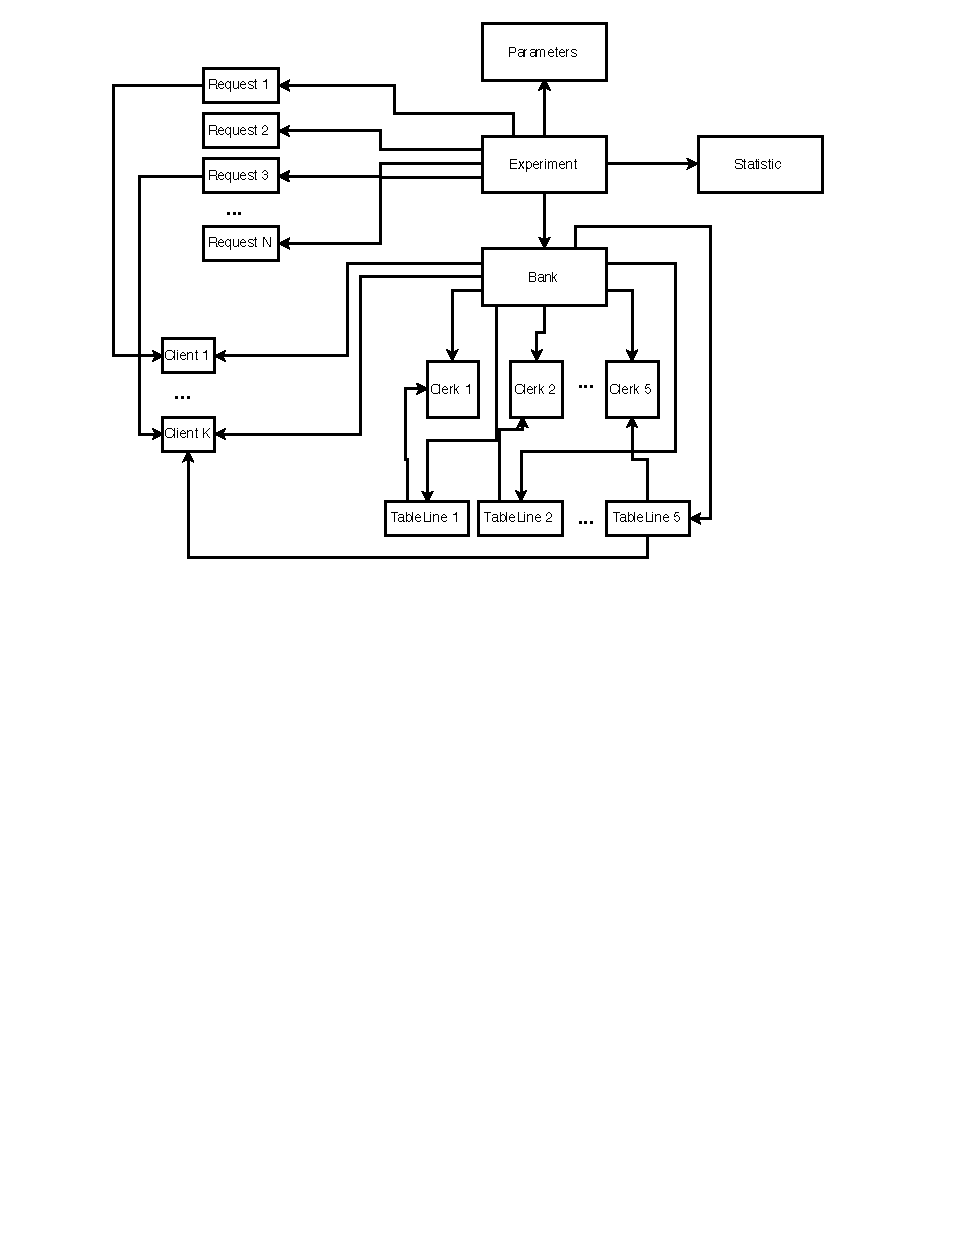
\includegraphics[width=180mm]{objects.pdf}
\newpage

\section{Инструментальные средства}
Язык разработки: \textit{Haskell}\\

Используемые библиотеки: \textit{Miso}

\section{Описание файловой структуры системы}
\textbf{Main.hs} --- точка входа для запуска проекта;\\

\textbf{Experiment.hs} --- обработка событий, отрисовка интерфейса;\\

\textbf{Model.hs} --- описание классов и реализация их методов;\\

\textbf{Constants.hs} --- используемые константы.\\
\newpage
\section{Пользовательский интерфейс}
 
Пользовательский интерфейс представляет собой единое окно для настройки, визуализации банка и отображения статистики эксперимента.\\

На экране отображены основные параметры, кнопки для их изменения и кнопки для управления эспериментом:\\

 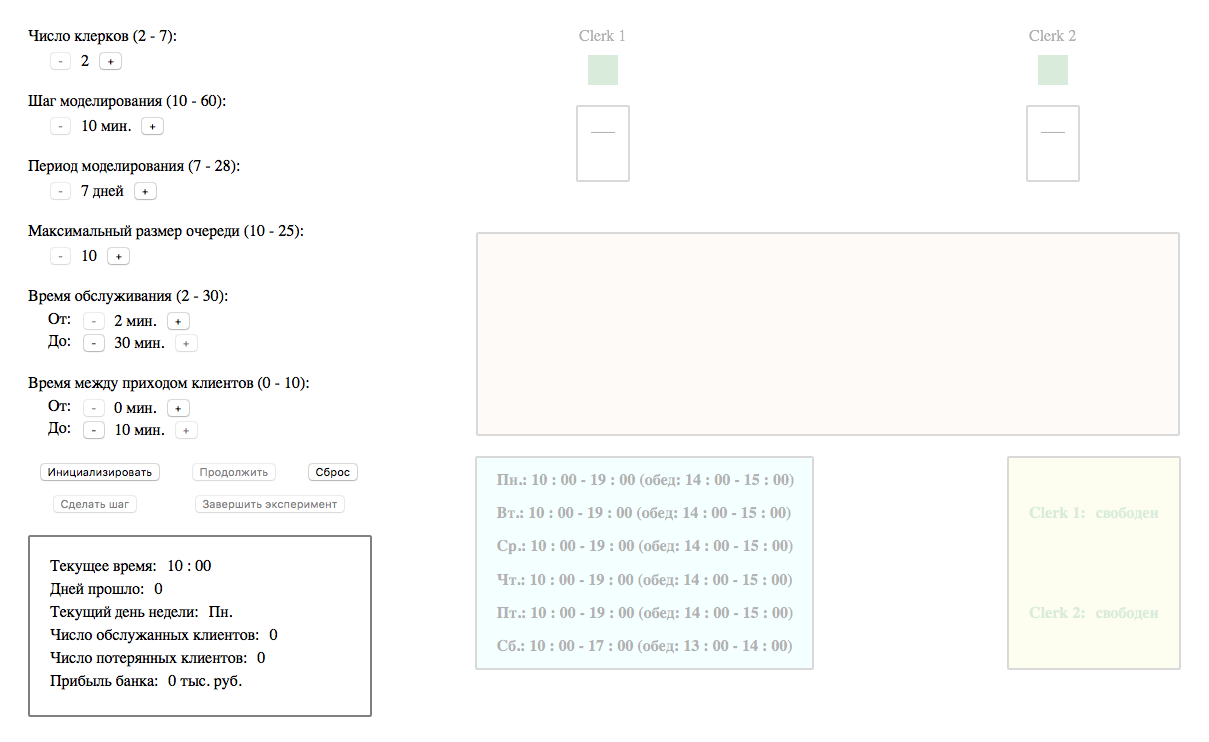
\includegraphics[width=150mm]{not_inited.png}\\
 
 Стоит отметить, что после инициализации эксперимента изменять параметры становится невозможным, за исключением параметра <<Шаг моделирования>>.\\
 
 \newpage
 
 Для начала эксперимента пользователю нужно нажать кнопку <<Инициализировать>>, и эксперимент начнет моделироваться в реальном времени (1 мин. $\sim$ 1 сек.):\\
 
 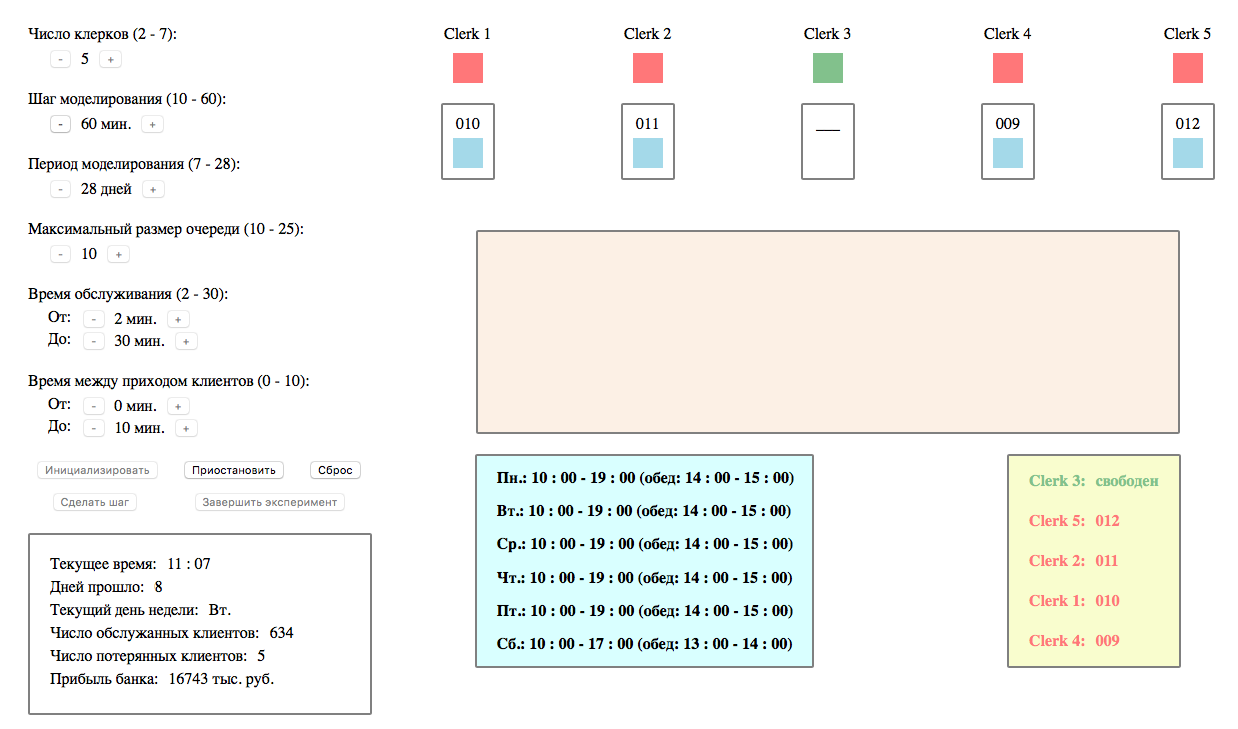
\includegraphics[width=150mm]{processing.png}\\

 \newpage
 
Эксперимент можно приостановить, нажав кнопку <<Приостановить>>:\\

 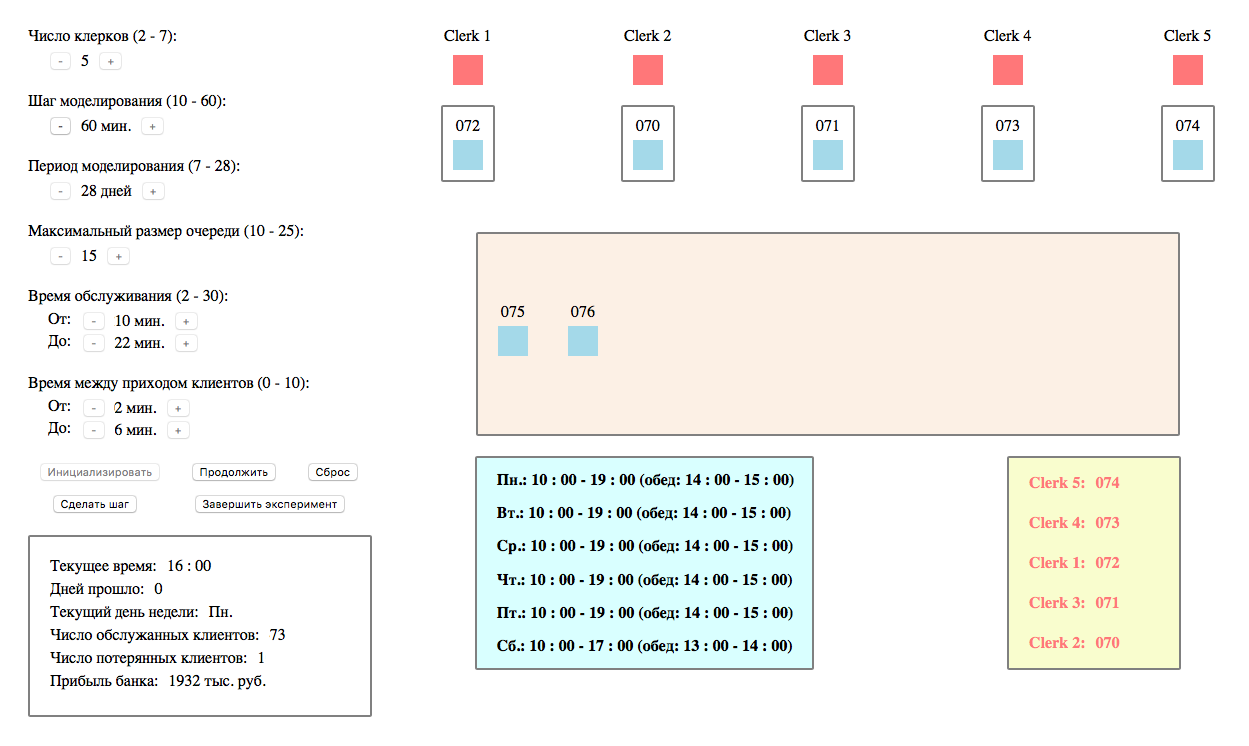
\includegraphics[width=150mm]{paused.png}\\

В данном состоянии можно смоделировать заданный в параметре <<Шаг моделирования>> промежуток времени, нажав кнопку <<Сделать шаг>>, смоделировать весь эксперимент до конца, нажав кнопку <<Завершить эксперимент>>, или же продолжить моделирование в реальном времени.\\

\newpage

В конце эксперимента будет выдан окончательный результат в таблице со статистикой:\\

 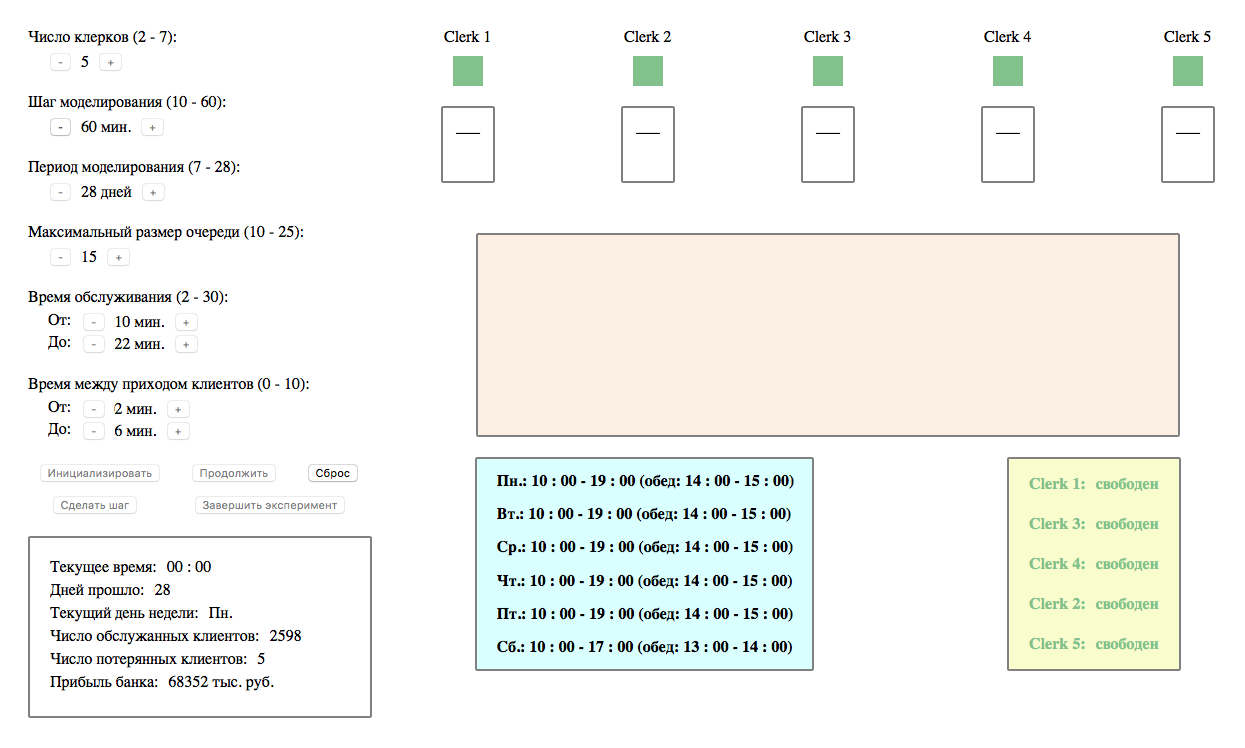
\includegraphics[width=150mm]{ended.png}\\

В любой момент эксперимента его можно сбросить к первоначальной конфигурации, нажав кнопку <<Сброс>>.\\

\newpage

\end{document}